\chapter{Caminos y circuitos}

Este capítulo trata de dos tipos de caminos en un grafo:
\begin{itemize}
    \item Un \key{camino euleriano} es un camino que visita cada arista
          solo una vez.
    \item Un \key{camino hamiltoniano} es un camino que visita cada nodo
          solo una vez.
\end{itemize}

Mientras que los caminos euleriano y hamiltoniano parecen conceptos
similares a primera vista, los problemas computacionales relacionados
a ellos son muy diferentes. Resulta que hay una simple regla que
determina si un grafo contiene un camino euleriano, y también hay un
algoritmo eficiente para encontrarlo si existe. De lo contrario,
revisar la existencia de un camino hamiltoniano es un problema NP-difícil,
y no se conoce un algoritmo eficiente para resolver el problema.

\section{Caminos eulerianos}

\index{camino euleriano}

Un \key{camino euleriano}\footnote{L. Euler estudió estos caminos en 1736
    cuando resolvió el famoso problema de los puentes de Königsberg. Este fue
    el nacimiento de la teoría de grafos.} es un camino que pasa por cada
arista exactamente una vez. Por ejemplo, el grafo
\begin{center}
    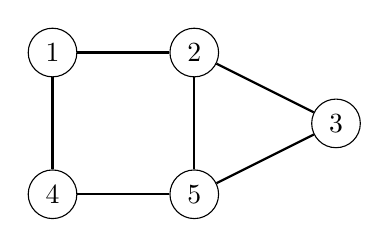
\begin{tikzpicture}[scale=0.9]
        \node[draw, circle] (1) at (1,5) {$1$};
        \node[draw, circle] (2) at (3,5) {$2$};
        \node[draw, circle] (3) at (5,4) {$3$};
        \node[draw, circle] (4) at (1,3) {$4$};
        \node[draw, circle] (5) at (3,3) {$5$};

        \path[draw,thick,-] (1) -- (2);
        \path[draw,thick,-] (2) -- (3);
        \path[draw,thick,-] (1) -- (4);
        \path[draw,thick,-] (3) -- (5);
        \path[draw,thick,-] (2) -- (5);
        \path[draw,thick,-] (4) -- (5);
    \end{tikzpicture}
\end{center}
tiene un camino euleriano del nodo 2 al nodo 5:
\begin{center}
    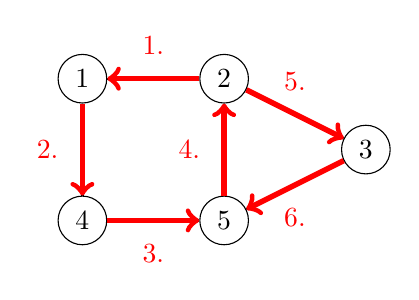
\begin{tikzpicture}[scale=0.9]
        \node[draw, circle] (1) at (1,5) {$1$};
        \node[draw, circle] (2) at (3,5) {$2$};
        \node[draw, circle] (3) at (5,4) {$3$};
        \node[draw, circle] (4) at (1,3) {$4$};
        \node[draw, circle] (5) at (3,3) {$5$};

        \path[draw,thick,-] (1) -- (2);
        \path[draw,thick,-] (2) -- (3);
        \path[draw,thick,-] (1) -- (4);
        \path[draw,thick,-] (3) -- (5);
        \path[draw,thick,-] (2) -- (5);
        \path[draw,thick,-] (4) -- (5);

        \path[draw=red,thick,->,line width=2pt] (2) -- node[font=\small,label={[red]north:1.}] {} (1);
        \path[draw=red,thick,->,line width=2pt] (1) -- node[font=\small,label={[red]left:2.}] {} (4);
        \path[draw=red,thick,->,line width=2pt] (4) -- node[font=\small,label={[red]south:3.}] {} (5);
        \path[draw=red,thick,->,line width=2pt] (5) -- node[font=\small,label={[red]left:4.}] {} (2);
        \path[draw=red,thick,->,line width=2pt] (2) -- node[font=\small,label={[red]north:5.}] {} (3);
        \path[draw=red,thick,->,line width=2pt] (3) -- node[font=\small,label={[red]south:6.}] {} (5);
    \end{tikzpicture}
\end{center}
\index{circuito euleriano}
Un \key{circuito euleriano} es un camino euleriano que comienza
y termina en el mismo nodo. Por ejemplo, el grafo
\begin{center}
    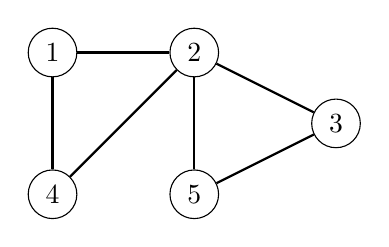
\begin{tikzpicture}[scale=0.9]
        \node[draw, circle] (1) at (1,5) {$1$};
        \node[draw, circle] (2) at (3,5) {$2$};
        \node[draw, circle] (3) at (5,4) {$3$};
        \node[draw, circle] (4) at (1,3) {$4$};
        \node[draw, circle] (5) at (3,3) {$5$};

        \path[draw,thick,-] (1) -- (2);
        \path[draw,thick,-] (2) -- (3);
        \path[draw,thick,-] (1) -- (4);
        \path[draw,thick,-] (3) -- (5);
        \path[draw,thick,-] (2) -- (5);
        \path[draw,thick,-] (2) -- (4);
    \end{tikzpicture}
\end{center}
tiene un circuito euleriano que comienza y termina en el nodo 1:
\begin{center}
    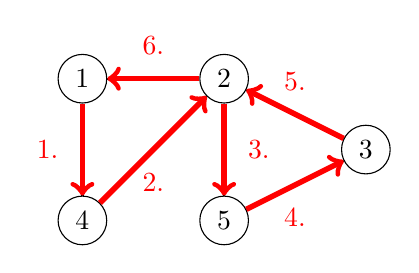
\begin{tikzpicture}[scale=0.9]
        \node[draw, circle] (1) at (1,5) {$1$};
        \node[draw, circle] (2) at (3,5) {$2$};
        \node[draw, circle] (3) at (5,4) {$3$};
        \node[draw, circle] (4) at (1,3) {$4$};
        \node[draw, circle] (5) at (3,3) {$5$};

        \path[draw,thick,-] (1) -- (2);
        \path[draw,thick,-] (2) -- (3);
        \path[draw,thick,-] (1) -- (4);
        \path[draw,thick,-] (3) -- (5);
        \path[draw,thick,-] (2) -- (5);
        \path[draw,thick,-] (2) -- (4);

        \path[draw=red,thick,->,line width=2pt] (1) -- node[font=\small,label={[red]left:1.}] {} (4);
        \path[draw=red,thick,->,line width=2pt] (4) -- node[font=\small,label={[red]south:2.}] {} (2);
        \path[draw=red,thick,->,line width=2pt] (2) -- node[font=\small,label={[red]right:3.}] {} (5);
        \path[draw=red,thick,->,line width=2pt] (5) -- node[font=\small,label={[red]south:4.}] {} (3);
        \path[draw=red,thick,->,line width=2pt] (3) -- node[font=\small,label={[red]north:5.}] {} (2);
        \path[draw=red,thick,->,line width=2pt] (2) -- node[font=\small,label={[red]north:6.}] {} (1);
    \end{tikzpicture}
\end{center}

\subsubsection{Existencia}

La existencia de los caminos y circuitos eulerianos depende del grado
de cada nodo. Para empezar, un grafo no dirigido tiene un camino euleriano
exactamente cuando todos los nodos pertenecen al mismo componente
conectado y
\begin{itemize}
    \item el grado de cada nodo es par \emph{o}
    \item el grado de \emph{exactamente} dos nodos es impar,
          y el resto es par.
\end{itemize}

En el primer caso, cada camino euleriano es también un circuito euleriano.
En el segundo caso, los nodos de grado impar son los inicios y finales
de un camino euleriano que no es un circuito euleriano.

Por ejemplo, en el grafo
\begin{center}
    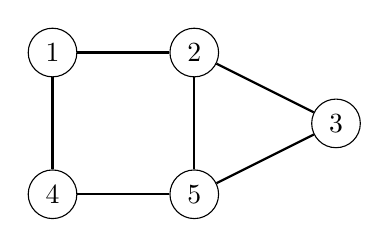
\begin{tikzpicture}[scale=0.9]
        \node[draw, circle] (1) at (1,5) {$1$};
        \node[draw, circle] (2) at (3,5) {$2$};
        \node[draw, circle] (3) at (5,4) {$3$};
        \node[draw, circle] (4) at (1,3) {$4$};
        \node[draw, circle] (5) at (3,3) {$5$};

        \path[draw,thick,-] (1) -- (2);
        \path[draw,thick,-] (2) -- (3);
        \path[draw,thick,-] (1) -- (4);
        \path[draw,thick,-] (3) -- (5);
        \path[draw,thick,-] (2) -- (5);
        \path[draw,thick,-] (4) -- (5);
    \end{tikzpicture}
\end{center}
los nodos 1, 3, y 4 tienen un grado de 2, y los nodos 2 y 5 tienen un
grado de 3. Exactamente dos nodos tienen un grado impar, por lo que
existe un camino euleriano entre los nodos 2 y 5, pero el grafo no
contiene un circuito euleriano.

En un grafo dirigido, nos concentramos en los grados de entrada y salida
de los nodos. Un grafo dirigido contiene un camino euleriano exactamente
cuando todos los nodos pertenecen al mismo componente conectado y
\begin{itemize}
    \item en cada nodo, el grado de entrada equivale el grado de salida, \emph{o}
    \item en un nodo, el grado de entrada es uno más que el grado de salida;
          en otro nodo, el grado de salida es uno más que el grado de entrada;
          y en todos los otros nodos, los grados de entrada y salida son iguales.
\end{itemize}

En el primer caso, cada camino euleriano es también un circuito euleriano,
y en el segundo caso, el grafo contiene un camino euleriano que comienza
en el nodo cuyo grado de salida es más grande y termina en el nodo cuyo
grado de entrada es más grande.

Por ejemplo, en el grafo
\begin{center}
    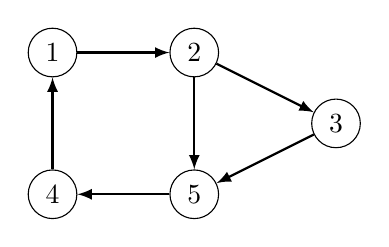
\begin{tikzpicture}[scale=0.9]
        \node[draw, circle] (1) at (1,5) {$1$};
        \node[draw, circle] (2) at (3,5) {$2$};
        \node[draw, circle] (3) at (5,4) {$3$};
        \node[draw, circle] (4) at (1,3) {$4$};
        \node[draw, circle] (5) at (3,3) {$5$};

        \path[draw,thick,->,>=latex] (1) -- (2);
        \path[draw,thick,->,>=latex] (2) -- (3);
        \path[draw,thick,->,>=latex] (4) -- (1);
        \path[draw,thick,->,>=latex] (3) -- (5);
        \path[draw,thick,->,>=latex] (2) -- (5);
        \path[draw,thick,->,>=latex] (5) -- (4);
    \end{tikzpicture}
\end{center}
los nodos 1, 3, y 4 tienen grado de salida y grado de entrada 1,
el nodo 2 tiene grado de entrada 1 y grado de salida 2, y el nodo 5
tiene grado de entrada 2 y grado de salida 1. Por ende, el grafo
contiene un camino euleriano del nodo 2 al nodo 5:
\begin{center}
    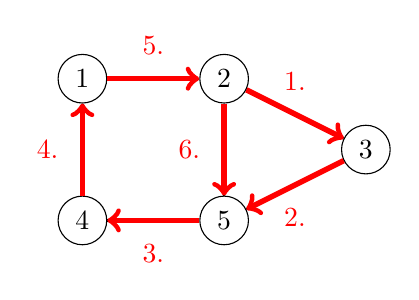
\begin{tikzpicture}[scale=0.9]
        \node[draw, circle] (1) at (1,5) {$1$};
        \node[draw, circle] (2) at (3,5) {$2$};
        \node[draw, circle] (3) at (5,4) {$3$};
        \node[draw, circle] (4) at (1,3) {$4$};
        \node[draw, circle] (5) at (3,3) {$5$};

        \path[draw,thick,-] (1) -- (2);
        \path[draw,thick,-] (2) -- (3);
        \path[draw,thick,-] (1) -- (4);
        \path[draw,thick,-] (3) -- (5);
        \path[draw,thick,-] (2) -- (5);
        \path[draw,thick,-] (4) -- (5);

        \path[draw=red,thick,->,line width=2pt] (2) -- node[font=\small,label={[red]north:1.}] {} (3);
        \path[draw=red,thick,->,line width=2pt] (3) -- node[font=\small,label={[red]south:2.}] {} (5);
        \path[draw=red,thick,->,line width=2pt] (5) -- node[font=\small,label={[red]south:3.}] {} (4);
        \path[draw=red,thick,->,line width=2pt] (4) -- node[font=\small,label={[red]left:4.}] {} (1);
        \path[draw=red,thick,->,line width=2pt] (1) -- node[font=\small,label={[red]north:5.}] {} (2);
        \path[draw=red,thick,->,line width=2pt] (2) -- node[font=\small,label={[red]left:6.}] {} (5);
    \end{tikzpicture}
\end{center}

\subsubsection{Algoritmo de Hierholzer}

\index{algoritmo de Hierholzer}

El \key{algoritmo de Hierholzer}\footnote{Este algoritmo fue publicado
    en 1873 después de la muerte de su autor \cite{hie73}.} es un
eficiente método para construir un circuito euleriano. El algoritmo
consiste de varias rondas, cada uno de las cuales añade nuevas aristas
al circuito. Por supuesto, asumimos que el grafo contiene un circuito
euleriano; de otro modo el algoritmo de Hierholzer no podría encontrarlo.

Primero, el algoritmo construye un circuito que contiene algunas
(no necesariamente todas) las aristas del grafo. Luego de esto, el
algoritmo extiende el circuito paso por paso añadiendo subcircuitos
a él. El proceso continúa hasta que todas las aristas se hayan
añadido al circuito.

El algoritmo extiende el circuito siempre encontrando un nodo $x$
que pertenece al circuito pero tiene una arista saliente que no esté
incluida en el circuito. El algoritmo construye un nuevo camino del
nodo $x$ que solo contiene aristas que todavía no están en el circuito.
Tarde o temprano, el camino volverá al nodo $x$, lo que crea un
subcircuito.

Si el grafo solamente contiene un camino euleriano, igualmente podemos
encontrarlo usando el algoritmo de Hierholzer si añadimos una arista
extra al grafo y la quitamos una vez que el circuito esté completo.
Por ejemplo, en un grafo no dirigido, añadimos la arista extra entre
los dos nodos de grado impar.

Ahora veremos cómo funciona el algoritmo de Hierholzer para construir
un circuito euleriano para un grafo no dirigido.

\subsubsection{Ejemplo}

Considera el siguiente grafo:
\begin{center}
    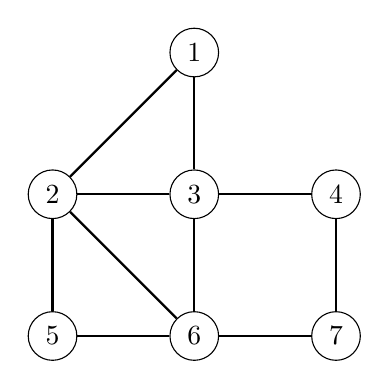
\begin{tikzpicture}[scale=0.9]
        \node[draw, circle] (1) at (3,5) {$1$};
        \node[draw, circle] (2) at (1,3) {$2$};
        \node[draw, circle] (3) at (3,3) {$3$};
        \node[draw, circle] (4) at (5,3) {$4$};
        \node[draw, circle] (5) at (1,1) {$5$};
        \node[draw, circle] (6) at (3,1) {$6$};
        \node[draw, circle] (7) at (5,1) {$7$};

        \path[draw,thick,-] (1) -- (2);
        \path[draw,thick,-] (1) -- (3);
        \path[draw,thick,-] (2) -- (3);
        \path[draw,thick,-] (2) -- (5);
        \path[draw,thick,-] (2) -- (6);
        \path[draw,thick,-] (3) -- (4);
        \path[draw,thick,-] (3) -- (6);
        \path[draw,thick,-] (4) -- (7);
        \path[draw,thick,-] (5) -- (6);
        \path[draw,thick,-] (6) -- (7);
    \end{tikzpicture}
\end{center}

Supongamos que el algoritmo primero crea un circuito que comienza en
el nodo 1. Un circuito posible es
$1 \rightarrow 2 \rightarrow 3 \rightarrow 1$:
\begin{center}
    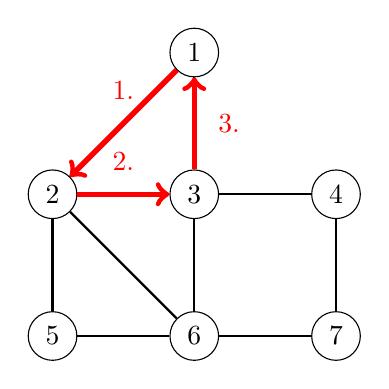
\begin{tikzpicture}[scale=0.9]
        \node[draw, circle] (1) at (3,5) {$1$};
        \node[draw, circle] (2) at (1,3) {$2$};
        \node[draw, circle] (3) at (3,3) {$3$};
        \node[draw, circle] (4) at (5,3) {$4$};
        \node[draw, circle] (5) at (1,1) {$5$};
        \node[draw, circle] (6) at (3,1) {$6$};
        \node[draw, circle] (7) at (5,1) {$7$};

        \path[draw,thick,-] (1) -- (2);
        \path[draw,thick,-] (1) -- (3);
        \path[draw,thick,-] (2) -- (3);
        \path[draw,thick,-] (2) -- (5);
        \path[draw,thick,-] (2) -- (6);
        \path[draw,thick,-] (3) -- (4);
        \path[draw,thick,-] (3) -- (6);
        \path[draw,thick,-] (4) -- (7);
        \path[draw,thick,-] (5) -- (6);
        \path[draw,thick,-] (6) -- (7);

        \path[draw=red,thick,->,line width=2pt] (1) -- node[font=\small,label={[red]north:1.}] {} (2);
        \path[draw=red,thick,->,line width=2pt] (2) -- node[font=\small,label={[red]north:2.}] {} (3);
        \path[draw=red,thick,->,line width=2pt] (3) -- node[font=\small,label={[red]east:3.}] {} (1);
    \end{tikzpicture}
\end{center}
Luego de esto, el algoritmo añade el subcircuito
$2 \rightarrow 5 \rightarrow 6 \rightarrow 2$ al circuito:
\begin{center}
    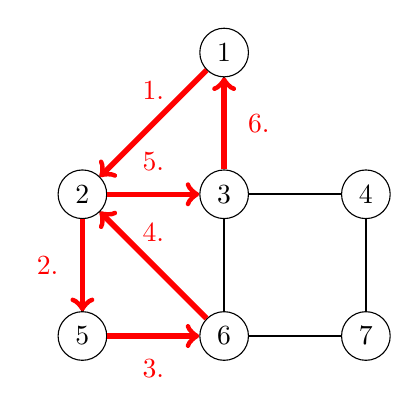
\begin{tikzpicture}[scale=0.9]
        \node[draw, circle] (1) at (3,5) {$1$};
        \node[draw, circle] (2) at (1,3) {$2$};
        \node[draw, circle] (3) at (3,3) {$3$};
        \node[draw, circle] (4) at (5,3) {$4$};
        \node[draw, circle] (5) at (1,1) {$5$};
        \node[draw, circle] (6) at (3,1) {$6$};
        \node[draw, circle] (7) at (5,1) {$7$};

        \path[draw,thick,-] (1) -- (2);
        \path[draw,thick,-] (1) -- (3);
        \path[draw,thick,-] (2) -- (3);
        \path[draw,thick,-] (2) -- (5);
        \path[draw,thick,-] (2) -- (6);
        \path[draw,thick,-] (3) -- (4);
        \path[draw,thick,-] (3) -- (6);
        \path[draw,thick,-] (4) -- (7);
        \path[draw,thick,-] (5) -- (6);
        \path[draw,thick,-] (6) -- (7);

        \path[draw=red,thick,->,line width=2pt] (1) -- node[font=\small,label={[red]north:1.}] {} (2);
        \path[draw=red,thick,->,line width=2pt] (2) -- node[font=\small,label={[red]west:2.}] {} (5);
        \path[draw=red,thick,->,line width=2pt] (5) -- node[font=\small,label={[red]south:3.}] {} (6);
        \path[draw=red,thick,->,line width=2pt] (6) -- node[font=\small,label={[red]north:4.}] {} (2);
        \path[draw=red,thick,->,line width=2pt] (2) -- node[font=\small,label={[red]north:5.}] {} (3);
        \path[draw=red,thick,->,line width=2pt] (3) -- node[font=\small,label={[red]east:6.}] {} (1);
    \end{tikzpicture}
\end{center}
Finalmente, el algoritmo añade el subcircuito
$6 \rightarrow 3 \rightarrow 4 \rightarrow 7 \rightarrow 6$ al circuito:
\begin{center}
    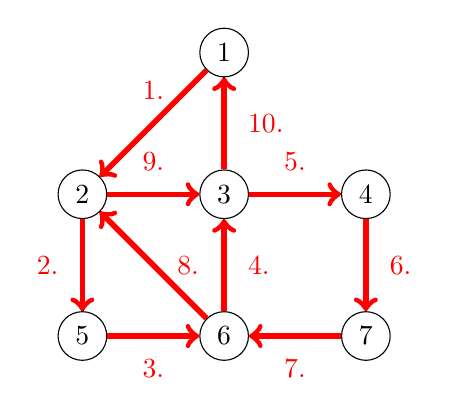
\begin{tikzpicture}[scale=0.9]
        \node[draw, circle] (1) at (3,5) {$1$};
        \node[draw, circle] (2) at (1,3) {$2$};
        \node[draw, circle] (3) at (3,3) {$3$};
        \node[draw, circle] (4) at (5,3) {$4$};
        \node[draw, circle] (5) at (1,1) {$5$};
        \node[draw, circle] (6) at (3,1) {$6$};
        \node[draw, circle] (7) at (5,1) {$7$};

        \path[draw,thick,-] (1) -- (2);
        \path[draw,thick,-] (1) -- (3);
        \path[draw,thick,-] (2) -- (3);
        \path[draw,thick,-] (2) -- (5);
        \path[draw,thick,-] (2) -- (6);
        \path[draw,thick,-] (3) -- (4);
        \path[draw,thick,-] (3) -- (6);
        \path[draw,thick,-] (4) -- (7);
        \path[draw,thick,-] (5) -- (6);
        \path[draw,thick,-] (6) -- (7);

        \path[draw=red,thick,->,line width=2pt] (1) -- node[font=\small,label={[red]north:1.}] {} (2);
        \path[draw=red,thick,->,line width=2pt] (2) -- node[font=\small,label={[red]west:2.}] {} (5);
        \path[draw=red,thick,->,line width=2pt] (5) -- node[font=\small,label={[red]south:3.}] {} (6);
        \path[draw=red,thick,->,line width=2pt] (6) -- node[font=\small,label={[red]east:4.}] {} (3);
        \path[draw=red,thick,->,line width=2pt] (3) -- node[font=\small,label={[red]north:5.}] {} (4);
        \path[draw=red,thick,->,line width=2pt] (4) -- node[font=\small,label={[red]east:6.}] {} (7);
        \path[draw=red,thick,->,line width=2pt] (7) -- node[font=\small,label={[red]south:7.}] {} (6);
        \path[draw=red,thick,->,line width=2pt] (6) -- node[font=\small,label={[red]right:8.}] {} (2);
        \path[draw=red,thick,->,line width=2pt] (2) -- node[font=\small,label={[red]north:9.}] {} (3);
        \path[draw=red,thick,->,line width=2pt] (3) -- node[font=\small,label={[red]east:10.}] {} (1);
    \end{tikzpicture}
\end{center}
Ahora todas las aristas están incluidas en el circuito, por lo que
hemos construido un circuito euleriano.

\section{Caminos hamiltonianos}

\index{camino hamiltoniano}

Un \key{camino hamiltoniano} es un camino que visita cada nodo del grafo
exactamente una vez. Por ejemplo, el grafo
\begin{center}
    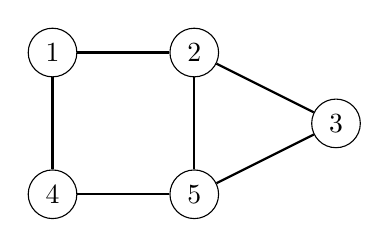
\begin{tikzpicture}[scale=0.9]
        \node[draw, circle] (1) at (1,5) {$1$};
        \node[draw, circle] (2) at (3,5) {$2$};
        \node[draw, circle] (3) at (5,4) {$3$};
        \node[draw, circle] (4) at (1,3) {$4$};
        \node[draw, circle] (5) at (3,3) {$5$};

        \path[draw,thick,-] (1) -- (2);
        \path[draw,thick,-] (2) -- (3);
        \path[draw,thick,-] (1) -- (4);
        \path[draw,thick,-] (3) -- (5);
        \path[draw,thick,-] (2) -- (5);
        \path[draw,thick,-] (4) -- (5);
    \end{tikzpicture}
\end{center}
contiene un camino hamiltoniano del nodo 1 al nodo 3:
\begin{center}
    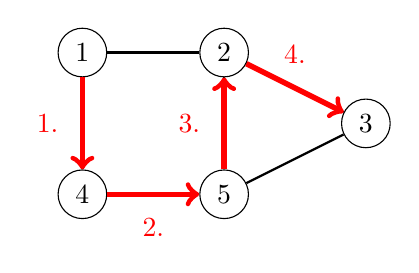
\begin{tikzpicture}[scale=0.9]
        \node[draw, circle] (1) at (1,5) {$1$};
        \node[draw, circle] (2) at (3,5) {$2$};
        \node[draw, circle] (3) at (5,4) {$3$};
        \node[draw, circle] (4) at (1,3) {$4$};
        \node[draw, circle] (5) at (3,3) {$5$};

        \path[draw,thick,-] (1) -- (2);
        \path[draw,thick,-] (2) -- (3);
        \path[draw,thick,-] (1) -- (4);
        \path[draw,thick,-] (3) -- (5);
        \path[draw,thick,-] (2) -- (5);
        \path[draw,thick,-] (4) -- (5);

        \path[draw=red,thick,->,line width=2pt] (1) -- node[font=\small,label={[red]left:1.}] {} (4);
        \path[draw=red,thick,->,line width=2pt] (4) -- node[font=\small,label={[red]south:2.}] {} (5);
        \path[draw=red,thick,->,line width=2pt] (5) -- node[font=\small,label={[red]left:3.}] {} (2);
        \path[draw=red,thick,->,line width=2pt] (2) -- node[font=\small,label={[red]north:4.}] {} (3);
    \end{tikzpicture}
\end{center}

\index{circuito hamiltoniano}

Si un camino hamiltoniano comienza y termina en el mismo nodo, se le
denomina \key{circuito hamiltoniano}. El grafo de arriba también contiene
un circuito hamiltoniano que comienza y termina en el nodo 1:
\begin{center}
    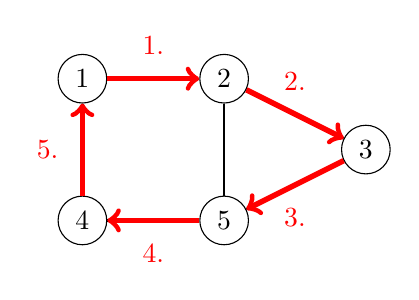
\begin{tikzpicture}[scale=0.9]
        \node[draw, circle] (1) at (1,5) {$1$};
        \node[draw, circle] (2) at (3,5) {$2$};
        \node[draw, circle] (3) at (5,4) {$3$};
        \node[draw, circle] (4) at (1,3) {$4$};
        \node[draw, circle] (5) at (3,3) {$5$};

        \path[draw,thick,-] (1) -- (2);
        \path[draw,thick,-] (2) -- (3);
        \path[draw,thick,-] (1) -- (4);
        \path[draw,thick,-] (3) -- (5);
        \path[draw,thick,-] (2) -- (5);
        \path[draw,thick,-] (4) -- (5);

        \path[draw=red,thick,->,line width=2pt] (1) -- node[font=\small,label={[red]north:1.}] {} (2);
        \path[draw=red,thick,->,line width=2pt] (2) -- node[font=\small,label={[red]north:2.}] {} (3);
        \path[draw=red,thick,->,line width=2pt] (3) -- node[font=\small,label={[red]south:3.}] {} (5);
        \path[draw=red,thick,->,line width=2pt] (5) -- node[font=\small,label={[red]south:4.}] {} (4);
        \path[draw=red,thick,->,line width=2pt] (4) -- node[font=\small,label={[red]left:5.}] {} (1);
    \end{tikzpicture}
\end{center}

\subsubsection{Existencia}

No se conoce un método eficiente para revisar si un grafo contiene un
camino hamiltoniano, y el problema es NP-difícil. No obstante, en algunos
casos especiales, podemos estar seguros de que un grafo contiene un
camino hamiltoniano.

Una simple observación es que si el grafo es completo, o sea, si hay una
arista entre cada par de nodos, también contiene un camino hamiltoniano.
También se han encontrado resultados más fuertes:

\index{teorema de Dirac}
\index{teorema de Ore}

\begin{itemize}
    \item El \key{teorema de Dirac}: si el grado de cada nodo es al menos
          $\displaystyle n/2$, el grafo contiene un camino hamiltoniano.
    \item El \key{teorema de Ore}: si la suma de los grados de cada
          par de nodos no adyacente es al menos $n$, el grafo contiene un
          camino hamiltoniano.
\end{itemize}

Una propiedad común en estos teoremas y otros resultados es que
garantizan la existencia de un camino hamiltoniano si el grafo contiene
\emph{un gran número} de aristas. Esto tiene sentido, ya que cuantas más
aristas contenga el grafo, más posibilidades hay de construir un camino
hamiltoniano.

\subsubsection{Construcción}

Debido a que no hay una manera eficiente de revisar si existe un
camino hamiltoniano, está claro que tampoco existe un método para
construir tal camino---sino podríamos simplemente intentar construir
el camino y ver si existe.

Una simple forma de encontrar un camino hamiltoniano es usando un
algoritmo de backtracking que revisa todas las formas posibles de
construir el camino. La complejidad temporal de tal algoritmo es
por lo menos $O(n!)$, porque existen $n!$ diferentes formas de elegir
el orden de $n$ nodos.

Una solución más eficiente se basa en la programación dinámica (ver
Capítulo 10.5). La idea es calcular valores de una función
$\texttt{posible}(S,x)$ donde $S$ es un subconjunto de nodos y $x$
es uno de los nodos. La función indica si existe un camino hamiltoniano
que visite los nodos de $S$ y termine en el nodo $x$. Es posible
implementar esta solución en $O(2^n n^2)$.

\section{Secuencias de De Bruijn}

\index{secuencia de De Bruijn}

Una \key{secuencia de De Bruijn} es una cadena que contiene cada cadena
de longitud $n$ exactamente una vez como subcadena, para un alfabeto
fijo de $k$ caracteres. La longitud de tal cadena es $k^n+n-1$ caracteres.
Por ejemplo, cuando $n=3$ y $k=2$, un ejemplo de una secuencia de
De Bruijn es \[0001011100.\]
Las subcadenas de esta cadena son:
000, 001, 010, 011, 100, 101, 110, y 111.

Resulta que cada secuencia de De Bruijn corresponde a un camino euleriano
en un grafo. La idea es construir un grafo donde cada nodo contiene una
cadena de $n-1$ caracteres y cada arista añade un carácter a la cadena.
El siguiente grafo corresponde a la situación de arriba:

\begin{center}
    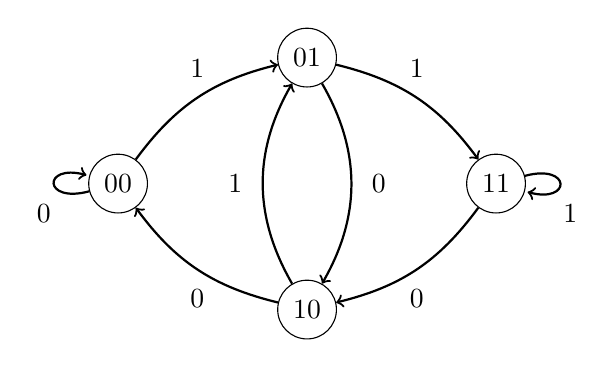
\begin{tikzpicture}[scale=0.8]
        \node[draw, circle] (00) at (-3,0) {00};
        \node[draw, circle] (11) at (3,0) {11};
        \node[draw, circle] (01) at (0,2) {01};
        \node[draw, circle] (10) at (0,-2) {10};

        \path[draw,thick,->] (00) edge [bend left=20] node[font=\small,label=1] {} (01);
        \path[draw,thick,->] (01) edge [bend left=20] node[font=\small,label=1] {} (11);
        \path[draw,thick,->] (11) edge [bend left=20] node[font=\small,label=below:0] {} (10);
        \path[draw,thick,->] (10) edge [bend left=20] node[font=\small,label=below:0] {} (00);

        \path[draw,thick,->] (01) edge [bend left=30] node[font=\small,label=right:0] {} (10);
        \path[draw,thick,->] (10) edge [bend left=30] node[font=\small,label=left:1] {} (01);

        \path[draw,thick,-] (00) edge [loop left] node[font=\small,label=below:0] {} (00);
        \path[draw,thick,-] (11) edge [loop right] node[font=\small,label=below:1] {} (11);
    \end{tikzpicture}
\end{center}

Un camino euleriano en este grafo corresponde a la cadena que contiene
todas las cadenas de longitud $n$. La cadena contiene los caracteres
del nodo inicial y todos los caracteres de las aristas. El nodo inicial
tiene $n-1$ caracteres y hay $k^n$ caracteres en las aristas, por lo que
la longitud de la cadena es $k^n+n-1$.

\section{Problema del caballo}

\index{problema del caballo}

El \key{problema del caballo} consiste en construir una secuencia de
movimientos del caballo en un tablero de ajedrez de $n \times n$
siguiendo las reglas del ajedrez tal que el caballo visita cada cuadrado
exactamente una vez. Un recorrido del caballo se denomina \emph{cerrado}
si el caballo finalmente vuelve al cuadrado inicial y, de lo contrario,
se lo llama \emph{abierto}.

Por ejemplo, aquí hay un recorrido de caballo abierto en un
tablero de $5 \times 5$:

\begin{center}
    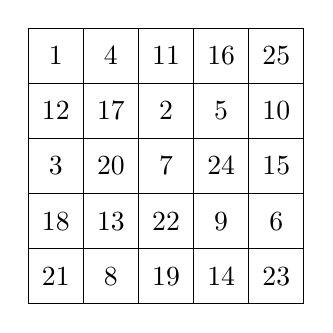
\begin{tikzpicture}[scale=0.7]
        \draw (0,0) grid (5,5);
        \node at (0.5,4.5) {$1$};
        \node at (1.5,4.5) {$4$};
        \node at (2.5,4.5) {$11$};
        \node at (3.5,4.5) {$16$};
        \node at (4.5,4.5) {$25$};
        \node at (0.5,3.5) {$12$};
        \node at (1.5,3.5) {$17$};
        \node at (2.5,3.5) {$2$};
        \node at (3.5,3.5) {$5$};
        \node at (4.5,3.5) {$10$};
        \node at (0.5,2.5) {$3$};
        \node at (1.5,2.5) {$20$};
        \node at (2.5,2.5) {$7$};
        \node at (3.5,2.5) {$24$};
        \node at (4.5,2.5) {$15$};
        \node at (0.5,1.5) {$18$};
        \node at (1.5,1.5) {$13$};
        \node at (2.5,1.5) {$22$};
        \node at (3.5,1.5) {$9$};
        \node at (4.5,1.5) {$6$};
        \node at (0.5,0.5) {$21$};
        \node at (1.5,0.5) {$8$};
        \node at (2.5,0.5) {$19$};
        \node at (3.5,0.5) {$14$};
        \node at (4.5,0.5) {$23$};
    \end{tikzpicture}
\end{center}

Un recorrido del caballo corresponde a un camino hamiltoniano en un grafo
cuyos nodos representan los cuadrados del tablero, y dos nodos están
conectados por una arista si un caballo puede moverse entre los dos
cuadrados según las reglas del ajedrez.

Una manera natural de construir un recorrido del caballo es utilizando
backtracking. La búsqueda puede hacerse más eficiente usando
\emph{heurísticas} que intentan guiar al caballo para encontrar un
recorrido completo rápidamente.

\subsubsection{Regla de Warnsdorf}

\index{heurística}
\index{regla de Warnsdorf}

La \key{regla de Warnsdorf} es una simple y efectiva heurística para
encontrar un recorrido del caballo.\footnote{Esta heurística fue
    propuesta en el libro de H. C. von Warnsdorf \cite{war23} en 1823.
    También existen algoritmos polinomiales para encontrar recorridos del
    caballo \cite{par97}, pero son más complicados.}
Utilizando la regla, es posible construir un recorrido eficientemente
incluso en un tablero grande. La idea es siempre mover el caballo
tal que termine en un cuadrado donde el número de movimientos posibles
sea tan \emph{pequeño} como sea posible.

Por ejemplo, en la siguiente situación, existen cinco cuadrados posibles
a los que el caballo puede moverse (cuadrados $a \ldots e$):
\begin{center}
    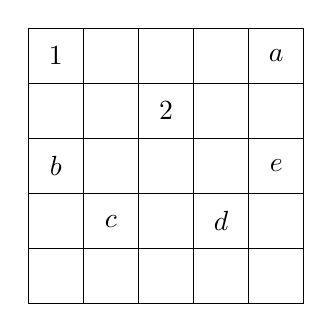
\begin{tikzpicture}[scale=0.7]
        \draw (0,0) grid (5,5);
        \node at (0.5,4.5) {$1$};
        \node at (2.5,3.5) {$2$};
        \node at (4.5,4.5) {$a$};
        \node at (0.5,2.5) {$b$};
        \node at (4.5,2.5) {$e$};
        \node at (1.5,1.5) {$c$};
        \node at (3.5,1.5) {$d$};
    \end{tikzpicture}
\end{center}
En esta situación, la regla de Warnsdorf mueve el caballo al cuadrado $a$,
porque luego de esta decisión, solo hay un movimiento posible. Las otras
decisiones moverían el caballo a cuadrados donde habría tres movimientos
posibles.
